\documentclass[a4paper]{article}
\usepackage[fontsize=13pt]{scrextend}
\usepackage[utf8]{vietnam}
\usepackage{amsmath}
\usepackage{amsfonts}
\usepackage{xcolor}
\usepackage{titlesec}
\usepackage{mdframed}
\usepackage{amssymb}
\usepackage{pgf,tikz,pgfplots}
\usepackage{graphicx}
\graphicspath{ {figures/} }
\usepackage{array}
\usepackage{cases}
\usepackage{listings}
\usepackage{tabulary}
\usepackage{color}
\usepackage{float} 
\usepackage{hyperref}
\usepackage{multirow}
\usepackage{minitoc}
\pgfplotsset{compat=1.5}
\usepackage{mathrsfs}
\usetikzlibrary{arrows, calc}
\usepackage{fancyhdr}
\pagestyle{fancy}
\pagestyle{empty}
\definecolor{dkgreen}{rgb}{0,0.6,0}
\definecolor{gray}{rgb}{0.5,0.5,0.5}
\definecolor{mauve}{rgb}{0.58,0,0.82}
\lstset{frame=tb,
  language=Python,
  aboveskip=3mm,
  belowskip=3mm,
  showstringspaces=false,
  columns=flexible,
  basicstyle={\small\ttfamily},
  numbers=none,
  numberstyle=\tiny\color{gray},
  keywordstyle=\color{blue},
  commentstyle=\color{dkgreen},
  stringstyle=\color{mauve},
  breaklines=true,
  breakatwhitespace=true,
  tabsize=3
}
\renewcommand{\listfigurename}{Danh sách hình}
\renewcommand{\listtablename}{Tables}
\newcommand{\tabitem}{~~\llap{\textbullet}~~}
\usepackage[left=2cm,right=2cm,top=2cm,bottom=2cm]{geometry}
\author{Nguyễn Văn Lộc}
\newmdenv[linecolor=black,skipabove=\topsep,skipbelow=\topsep,
leftmargin=-5pt,rightmargin=-5pt,
innerleftmargin=5pt,innerrightmargin=5pt]{mybox}
\hypersetup{
    colorlinks=true,
    linkcolor=blue,
    filecolor=magenta,      
    urlcolor=red,
    pdftitle={Report},   
}
\begin{document}
\fancyhf{}
\lhead{Báo cáo đồ án môn học Toán ứng dụng và thống kê $-$ Đồ án 1}
\chead{}
\rhead{Bài toán 2}
\cfoot{\thepage}
\rfoot{}
\lfoot{}
\pagestyle{fancy}
\begin{titlepage}
\begin{mybox}
\begin{center}
\fontsize{12}{12}\selectfont
\textbf{ĐẠI HỌC QUỐC GIA THÀNH PHỐ HỒ CHÍ MINH}\\
\textbf{TRƯỜNG ĐẠI HỌC KHOA HỌC TỰ NHIÊN}\\
\textbf{KHOA CÔNG NGHỆ THÔNG TIN}
\end{center}
\vskip 1 cm
\begin{figure}[H]
\begin{center}

\includegraphics[scale=0.25]{images/logo}
\end{center}
\end{figure}
\vskip 1 cm
\begin{center}
\fontsize{18}{14}\selectfont
\textbf{ĐỒ ÁN MÔN HỌC}\\
\fontsize{26}{16}\selectfont
\textbf{TOÁN ỨNG DỤNG VÀ THỐNG KÊ}\\
\fontsize{18}{12}\selectfont
\textbf{ĐỀ TÀI: Bài toán khí hậu}\\
\textbf{Bài toán 2: Dự báo dữ liệu về nhiệt độ}
\end{center}
\vskip 1 cm
\fontsize{14}{12}\selectfont
\textbf{Giảng viên lý thuyết:} PGS.TS Nguyễn Đình Thúc\\
\textbf{Lớp:} 20TN\\
\textbf{Thành viên thực hiện:}
\begin{itemize}
\item 20120131 $-$ Nguyễn Văn Lộc
\item 20120536 $-$ Võ Trọng Nghĩa
\item 20120572 $-$ Nguyễn Kiều Minh Tâm
\end{itemize}
\vskip 3 cm
\begin{center}
\textbf{THÀNH PHỐ HỒ CHÍ MINH, THÁNG 4 NĂM 2022}
\end{center}
\end{mybox}
\end{titlepage}

\section*{Lời nói đầu}
Hiện nay, biến đổi khí hậu đang là một chủ đề nhận được sự quan tâm trên toàn thế giới. Nhiều tổ chức liên chính phủ như Ủy ban Liên chính phủ về Biến đổi Khí hậu (IPCC) được lập ra nhằm tìm kiếm những giải pháp cho tình trạng này. Trong đó, tình trạng nóng lên toàn cầu (global warming) nổi lên như một trong những vấn đề bức thiết nhất. Nhận thấy được tầm quan trọng này, nhóm chúng em quyết định làm bài toán về phân tích và dự đoán nhiệt độ trung bình năm ở một số nơi trên Trái Đất, nhằm giúp đưa ra những giải pháp phù hợp.
\begin{flushright}
Thành phố Hồ Chí Minh, tháng 4 năm 2022
\end{flushright} 
\newpage

\tableofcontents
\listoffigures
\listoftables
\newpage



\section{Đặt vấn đề}
\subsection{Xác định và hình thức hóa mục tiêu của bài toán}
\textbf{Bài toán:} Dự báo nhiệt độ trung bình năm ở 5 trạm khí tượng theo dữ liệu của Cơ quan Quản lý Khí quyển và Đại dương Quốc gia Hoa Kỳ, bao gồm:
\begin{itemize}
\item \textbf{Trạm 1:} Trạm Lieksa Lampela ở Phần Lan (FIE00144982).
\item \textbf{Trạm 2:} Trạm Jena Sternwarte ở Đức (GM000004204).
\item \textbf{Trạm 3:} Trạm Den Helder 1 ở Hà Lan (NLM00006235).
\item \textbf{Trạm 4:} Trạm Uppsala Aut ở Thụy Điển (SWE00139148).
\item \textbf{Trạm 5:} Trạm New York City's Central Park ở Hoa Kỳ (USW00094728).
\end{itemize}
\textbf{Hình thức hóa mục tiêu của bài toán:} dùng biểu đồ phân tán, tìm các hệ số hồi quy.

\subsection{Dạng bài toán}
Bài toán này thuộc dạng bài toán \textbf{Dự đoán} (từ dữ liệu hiện có trong hiện tại và quá khứ để đưa ra dự đoán dữ liệu trong tương lai chưa biết).

\subsection{Đối tượng được chọn cho bài toán}
Dữ liệu về nhiệt độ trung bình năm của 5 trạm nêu trên.\\
Cột TAVG của các  tập tin \textbf{FIE00144982.csv}, \textbf{GM000004204.csv}, \textbf{NLM00006235.csv}, \textbf{SWE00139148.csv}, \textbf{USW00094728.csv}  trong thư mục \textbf{gsoy-latest}, lấy từ \href{https://www.ncei.noaa.gov/data/gsoy/archive/}{dataset về Global Summary of the Year của NOAA}.

\subsection{Phạm vi, mức độ, quy mô của bài toán}
Theo không gian: dữ liệu được xử lý trong bài toán đại diện cho 5 bang/tỉnh ở 5 quốc gia khác nhau.\\
Theo thời gian: dữ liệu được thu thập trong vòng 30 năm, từ năm 1991 đến năm 2020.

\section{Thu thập và xử lý dữ liệu}
\subsection{Thu thập dữ liệu}
Dữ liệu xử lý trong bài toán này được thu thập từ dữ liệu của Cơ quan Quản lý Khí quyển và Đại dương Quốc gia Hoa Kỳ (NOAA), phần dữ liệu tổng hợp theo năm (Global Summary of the Year).

\subsection{Xử lý dữ liệu}
\subsubsection{Trích xuất dữ liệu}
Dữ liệu nhiệt độ trung bình năm từ các tập tin được trích xuất thành các tập dữ liệu \textbf{data0.csv}, \textbf{data1.csv}, \textbf{data2.csv}, \textbf{data3.csv}, \textbf{data4.csv}, theo thứ tự được nêu ra bên trên nhờ các hàm của module \lstinline{pandas}.
\subsubsection{Xử lý phần dữ liệu bị khuyết}
Dữ liệu từ tập tin gốc đầu tiên (tập tin \textbf{FIE00144982.csv}) bị khuyết phần dữ liệu của năm 2009., do đó, nhóm chúng em đã tìm cách "điền" vào những ô bị khuyết này. Nhiệt độ trung bình năm của năm 2009 trong tập tin này được tính bằng trung bình cộng của nhiệt độ trung bình năm 2008 và nhiệt độ trung bình năm 2010.\\
\begin{figure}[H]
\center{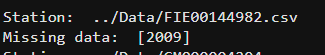
\includegraphics[scale=1]{images/missing.png}}
\caption{Phần dữ liệu bị khuyết}
\end{figure}

\section{Phân tích, đánh giá và kết luận}
Sau khi được tiền xử lý, dữ liệu được trực quan hóa (visualized)thành biểu đồ phân tán nhờ hàm hỗ trợ của module \lstinline{matplotlib}.

\subsection{Biểu đồ phân tán của dữ liệu}
Biểu đồ phân tán về nhiệt độ trung bình năm đo được tại 5 trạm trên như sau:
\begin{figure}[H]
\centering{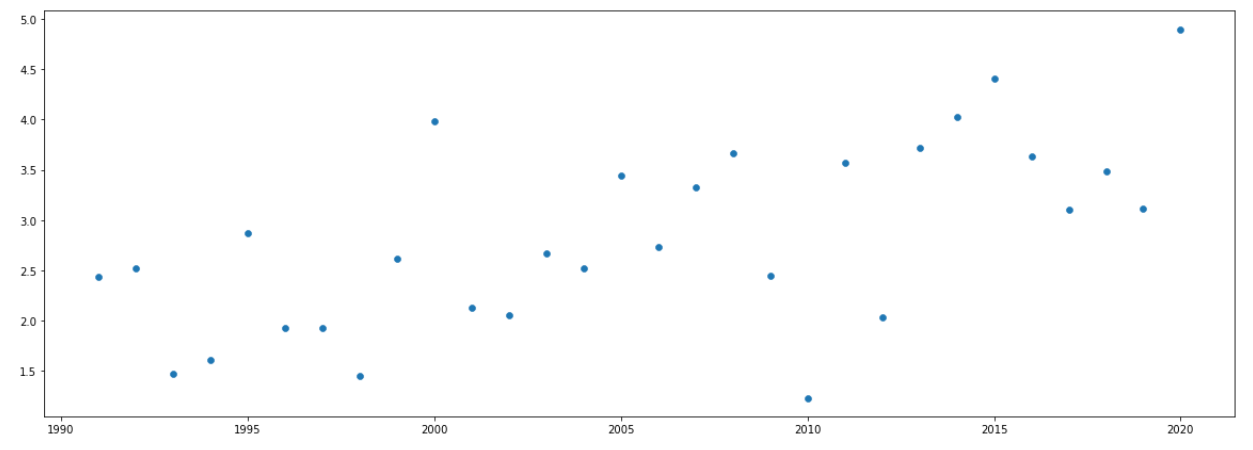
\includegraphics[scale=0.65]{images/scatter/station1}}
\caption{Biểu đồ phân tán dữ liệu của trạm 1}
\end{figure}

\begin{figure}[H]
\centering{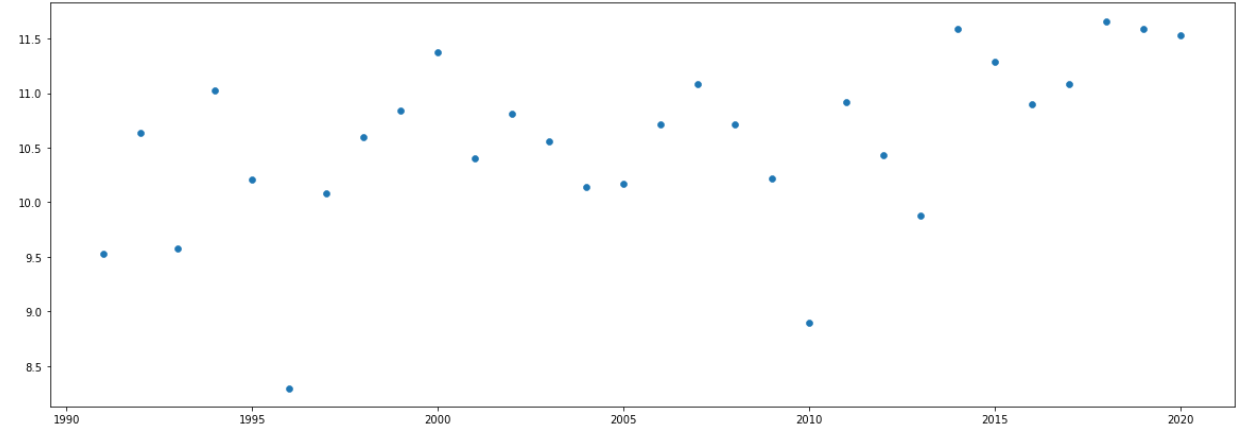
\includegraphics[scale=0.65]{images/scatter/station2}}
\caption{Biểu đồ phân tán dữ liệu của trạm 2}
\end{figure}

\begin{figure}[H]
\centering{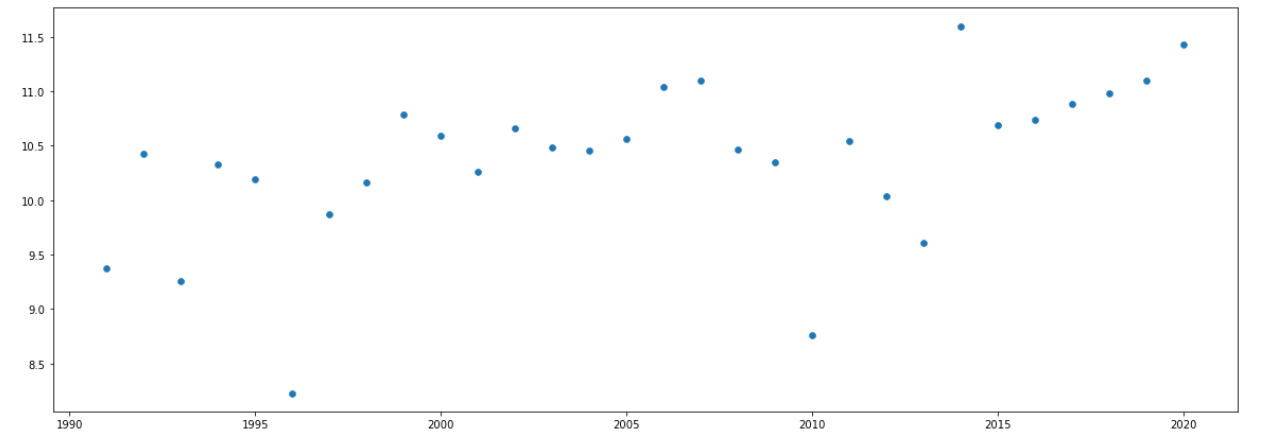
\includegraphics[scale=0.65]{images/scatter/station3}}
\caption{Biểu đồ phân tán dữ liệu của trạm 3}
\end{figure}

\begin{figure}[H]
\centering{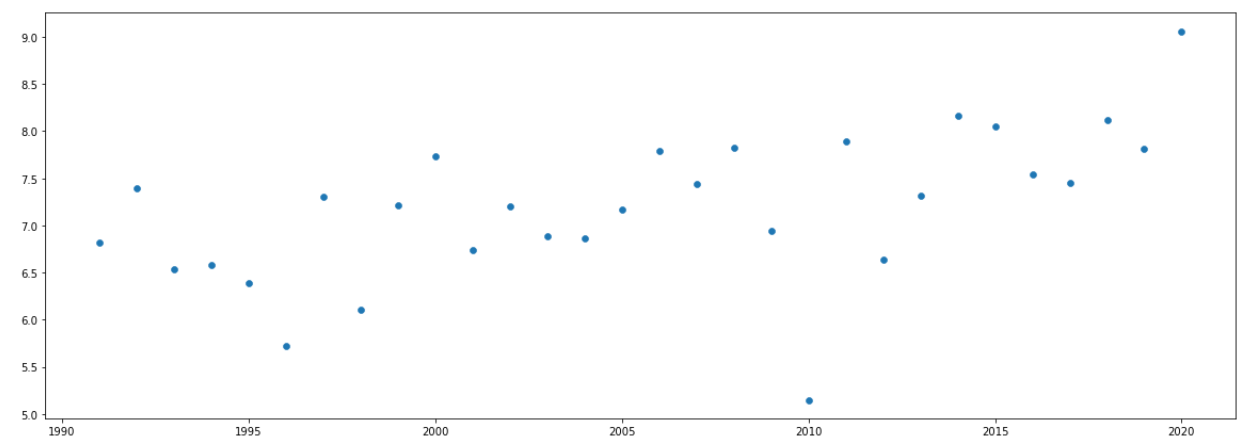
\includegraphics[scale=0.65]{images/scatter/station4}}
\caption{Biểu đồ phân tán dữ liệu của trạm 4}
\end{figure}

\begin{figure}[H]
\centering{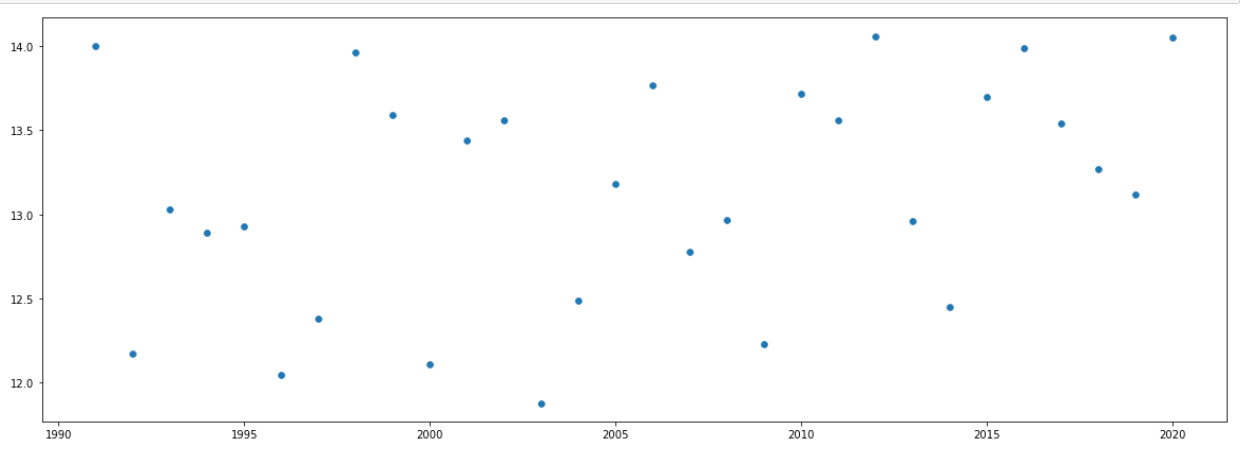
\includegraphics[scale=0.65]{images/scatter/station5}}
\caption{Biểu đồ phân tán dữ liệu của trạm 5}
\end{figure}

\subsection{Tìm mô hình}
Mô hình được chọn để dùng là mô hình \textbf{hồi quy} (regression). Đây là một mô hình khá thường gặp trong các bài toán dự đoán.\\ 
Dựa vào sự phân bổ của dữ liệu về nhiệt độ trung bình năm ở 5 trạm, hàm hồi quy $f \left( x \right)$ được chọn từ tổ hợp có giá trị r-squared lớn nhất với các hệ số thích hợp từ những hàm ${f_1}\left( x \right) = 1,$ ${f_2}\left( x \right) = x,$ ${f_3}\left( x \right) = {x^2},$ ${f_4}\left( x \right) = {x^3},$ ${f_5}\left( x \right) = {x^4},$ ${f_6}\left( x \right) = \ln \left( x \right),$ ${f_7}\left( x \right) = \sin \left( x \right)$ và ${f_8}\left( x \right) = \ln \left( x \right) \cdot \sin \left( x \right).$\\
Các hệ số của mô hình hồi quy được tìm như sau:\\
$x_1, x_2, ..., x_N$ là giá trị của các năm.\\
$Y = \left[ {\begin{array}{*{20}{c}}
  {{y_1}} \\ 
  {{y_2}} \\ 
   \vdots  \\ 
  {{y_N}} 
\end{array}} \right] \in {\mathbb{R}^N}$ là các giá trị nhiệt độ trung bình năm được chọn.\\
${f_1}\left( x \right),{f_2}\left( x \right), \ldots ,{f_p}\left( x \right)$ là các hàm được chọn cho mô hình.\\
$A = \left[ {\begin{array}{*{20}{c}}
  {{f_1}\left( {{x_1}} \right)}&{{f_2}\left( {{x_1}} \right)}& \ldots &{{f_p}\left( {{x_1}} \right)} \\ 
  {{f_1}\left( {{x_2}} \right)}&{{f_2}\left( {{x_2}} \right)}& \ldots &{{f_p}\left( {{x_2}} \right)} \\ 
   \vdots & \vdots & \vdots & \vdots  \\ 
  {{f_1}\left( {{x_N}} \right)}&{{f_2}\left( {{x_N}} \right)}& \ldots &{{f_p}\left( {{x_N}} \right)} 
\end{array}} \right] \in {\mathbb{R}^{N \times p}}.$\\
$\theta  = \left[ {\begin{array}{*{20}{c}}
  {{\theta _1}} \\ 
  {{\theta _2}} \\ 
   \vdots  \\ 
  {{\theta _p}} 
\end{array}} \right] \in {\mathbb{R}^p}$ là ma trận các hệ số của mô hình hồi quy.
Khi đó,
$${\theta _0} = {\left( {{A^T}A} \right)^{ - 1}}{A^T}Y.$$
Đoạn code tìm mô hình hồi quy như sau và vẽ đường hồi quy như sau:
\begin{lstlisting}
from itertools import chain, combinations
from sklearn.metrics import r2_score
def model_generate(_col):
    return [
            (_col, 'x', lambda x: x),
            (np.power(_col, 2), 'x^2', lambda x: np.power(x, 2)),
            (np.power(_col, 3), 'x^3', lambda x: np.power(x, 3)),
            (np.power(_col, 4), 'x^4', lambda x: np.power(x, 4)),
            (np.log(_col), 'log(x)', lambda x: np.log(x)),
            (np.sin(_col), 'sin(x)', lambda x: np.sin(x)),
            (np.multiply(np.sin(_col), np.log(_col)), 'log(x) * sin(x)', 
             lambda x: np.multiply(np.sin(x), np.log(x)))
    ]
    
def powerset(iterable):
    "powerset([1,2,3]) --> (1,) (2,) (3,) (1,2) (1,3) (2,3) (1,2,3)"
    s = list(iterable)
    return chain.from_iterable(combinations(s, r) for r in range(1, len(s)+1))

def calculate_theta(A, y):
    return np.linalg.inv(A.T * A) * A.T * y

def find_model(x, y):
    N = x.shape[0] # get number of rows
    _best_r2 = -np.Inf
    _best_model = None
    _best_theta = None
    _best_model_as_text = None
    for _model in powerset(model_generate(x)):
        A = np.ones((N, 1))
        for _elem in _model:
            A = np.concatenate((A, _elem[0]), axis = 1) # Merge columns
        try:
            theta = calculate_theta(A, y)
            y_hat = A * theta
            r2 = r2_score(np.squeeze(np.asarray(y, dtype=np.float64)), 
                            np.squeeze(np.asarray(y_hat, dtype=np.float64)))
            if _best_r2 < r2:
                _best_model = [item[2] for item in _model]
                _best_model_as_text = [item[1] for item in _model]
                _best_r2 = r2
                _best_theta = theta
        except:
            continue
    _text = ""
    _text += str(float(_best_theta[0])) + " + " 
    _text += "".join([str(np.round(a[0], 5)) + "*" + b + " + " 
                      for a,b in zip(np.asarray(_best_theta[1:]), _best_model_as_text)])[:-2]
    return (_best_r2, _text, _best_model, _best_theta)

def eval_value(_model, _theta, x):
    result = float(_theta[0])
    for model, theta in (zip(_model, _theta[1:])):
        result = result + float(model(x)) * float(theta)
    return result

def regression(file_name):
    # regression model
    df = pd.read_csv(file_name)
    x = np.matrix(np.arange(1991, 2020 + 1), dtype = np.float64).T # create N * 1 matrix
    y = np.matrix(list(df.iloc[:]['Temperature']), dtype = np.float64).T # create N * 1 matrix
    plt.scatter(np.squeeze(np.asarray(x)), 
                np.squeeze(np.asarray(y)), 
                linewidths=0.6)
    
    
    _r2, _text, _model, _theta = find_model(x, y)
    print(f"Best r2: {_r2}")
    print(f"Model: {_text}")

    x_test = np.linspace(1990, 2050, 200)
    y_test = np.array([eval_value(_model, _theta, _x) for _x in x_test])
    plt.plot(x_test, y_test)
    plt.show()
\end{lstlisting}

\subsubsection{Mô hình cụ thể của từng trạm}
Sau khi được chọn lọc, so sánh bởi các giá trị r-squared, các mô hình được chọn cho từng trạm như sau:
\begin{itemize}
\item Trạm 1: $ - 428760.8877986716 + 572.43424x  - 0.21496{x^2} + 336.39369\sin \left( x \right) - 44.23939\ln (x)\sin \left( x \right).$ Giá trị r-squared tương ứng là: $0.4152716333306189.$
\item Trạm 2: $ - 2240889.587199211 + 2981.88199x - 1.11596{x^2} + 474.80371*\sin \left( x \right) - 62.40748\ln \left( x \right)\sin \left( x \right).$ Giá trị r-squared tương ứng là: $0.43883419511592425.$
\item Trạm 3: $ - 2110487.082359817 + 2806.3352x - 1.04951{x^2} + 405.11019\sin \left( x \right) +  - 53.25191\ln \left( x \right)\sin \left( x \right).$ Giá trị r-squared tương ứng là: $0.3831435591080794.$
\item Trạm 4: $ - 1096522.0636323318 + 1461.34733x - 0.54775{x^2} + 207.56986\sin \left( x \right) - 27.28003\ln \left( x \right)\sin \left( x \right).$ Giá trị r-squared tương ứng là: $0.3877112193377744.$
\item Trạm 5: $91696.26412356505 + 6.95143x - 13891.27228\ln \left( x \right) + 120.21781\sin \left( x \right) - 15.79415\ln \left( x \right)\sin \left( x \right).$ Giá trị r-squared tương ứng là: $0.15745734304409686.$
\end{itemize}

\subsubsection{Kết quả dự đoán}
\begin{figure}[H]
\center{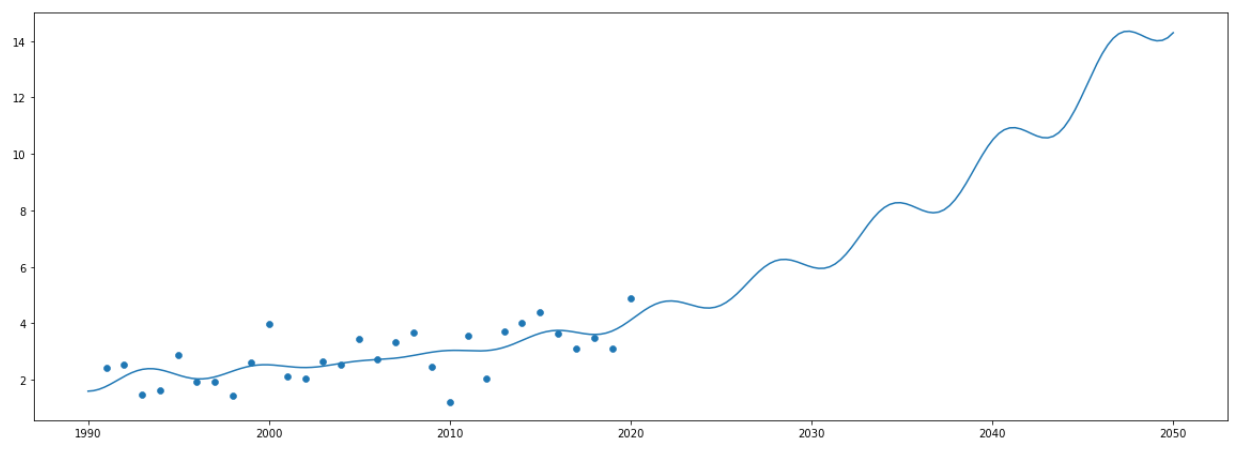
\includegraphics[scale=0.7]{images/result/res1}}
\caption{Kết quả ở trạm 1}
\end{figure}

\begin{figure}[H]
\center{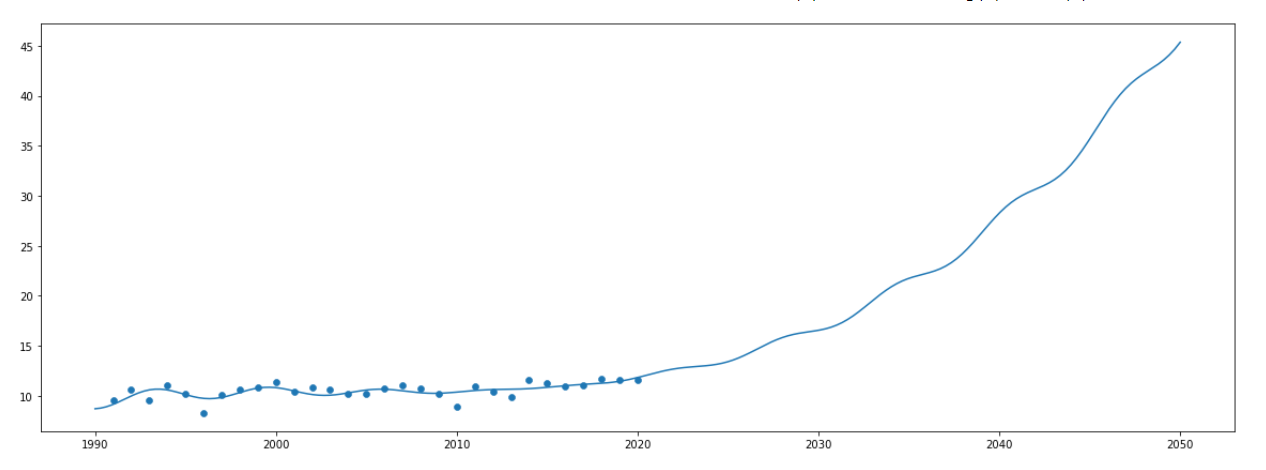
\includegraphics[scale=0.7]{images/result/res2}}
\caption{Kết quả ở trạm 2}
\end{figure}

\begin{figure}[H]
\center{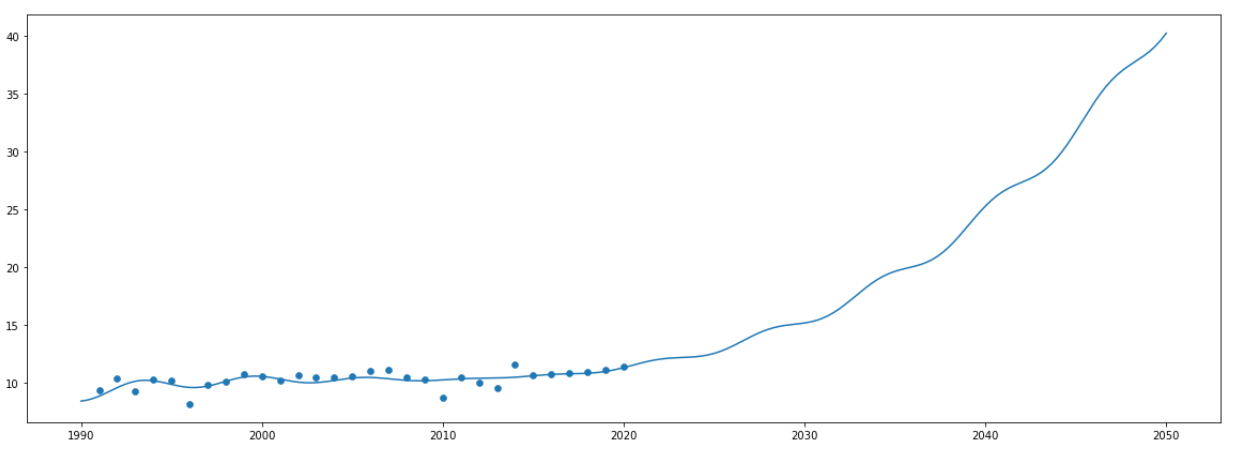
\includegraphics[scale=0.7]{images/result/res3}}
\caption{Kết quả ở trạm 3}
\end{figure}

\begin{figure}[H]
\center{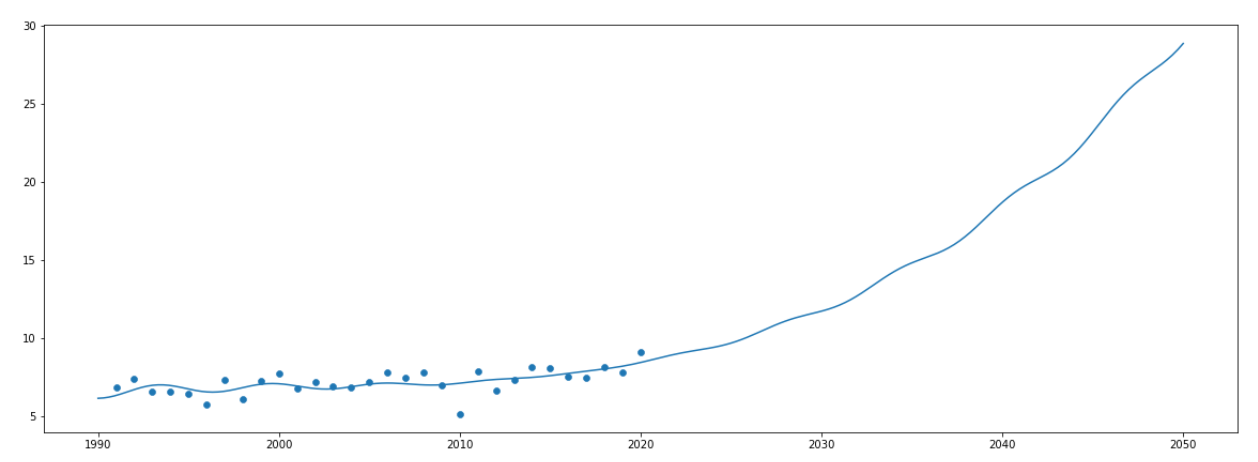
\includegraphics[scale=0.7]{images/result/res4}}
\caption{Kết quả ở trạm 4}
\end{figure}

\begin{figure}[H]
\center{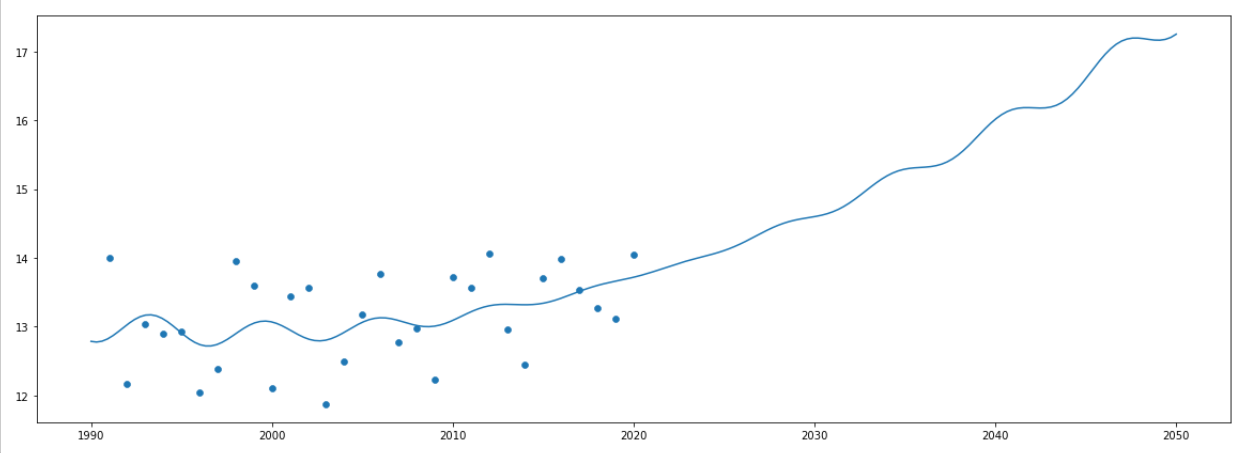
\includegraphics[scale=0.7]{images/result/res5}}
\caption{Kết quả ở trạm 5}
\end{figure}

Từ những kết quả được đưa ra từ mô hình hồi quy nêu trên, có thể thấy, nhiệt độ trung bình năm ở các địa điểm này đang dần tăng lên, nhất là kể từ khi máy tính trở nên bùng nổ vơi Cuộc Cách mạng Công ngiệp 4.0. Thậm chí, nhiệt độ trung bình năm ở một vài trạm có thể tăng gấp đôi vào năm 2050. Đây là hồi chuông báo động to lớn đối với toàn nhân loại về vấn đề biến đổi khí hậu, mà cá thể trong bài toán này là sự nóng lên toàn cầu, đặt ra một yêu cầu khẩn thiết về việc đưa ra những giải pháp thiết thực và kịp thời để giảm thiểu tình trạng nhiệt độ trung bình năm tăng cao.\\
Như vậy, bằng việc khảo sát một vài trạm khí tượng nằm rải rác khu vực Châu Âu và Bắc Mỹ, ta có thể thấy nhiệt độ trung bình năm đang có xu hướng tăng lên đáng báo động, đòi hỏi những biện pháp cấp bách từ các Chính phủ.
\newpage

\section*{Lời cảm ơn}
Trong quá trình thực hiện đồ án này, chúng em đã nhận được những bài giảng tận tâm, chi tiết về các phương pháp của Thầy Nguyễn Đình Thúc. Bên cạnh đó là những sự hướng dẫn của các Thầy, Cô trợ giảng cho môn học Toán ứng dụng và thống kê. Chúng em xin cảm ơn các Thầy, Cô.\\
Ngoài ra, chúng em cũng xin cảm ơn các bạn trong lớp đã đưa ra những chỉ dẫn, góp ý trong quá trình chúng em thực hiện đồ án.
\begin{flushright}
Thành phố Hồ Chí Minh, tháng 4 năm 2022
\end{flushright} 
\end{document}